\section{Auswertung}
\label{sec:Auswertung}
%Siehe \autoref{fig:plot}!

\subsection{Moden}
In diesem Teil werden die Moden mithilfe eine Oszilloskop untersucht.
Die aufgenommenen Werte zu zu den Moden sind in \autoref{tab:moden_messwerte} gelistet.
%tabelle messwerte
\begin{table}
    \centering
    \caption{Messwerte zu den drei Moden, wobei der erste Wert das Maximum beschreibt und die anderen beiden den Punkt links bzw. rechts vom Maximum bei dem die Spannung die hälfte des Maximums beträgt.}
    \begin{tabular}{c c c}
        \toprule
        Modennr. & $U \,/\, V$ & $A \,/\, V$ \\
        \midrule
        1 & $220$ & $31.25$ \\
        & $205$ & $0$ \\
        & $240$ & $0$ \\
        \hline
        2 & $140$ & $21.25$ \\
        & $120$ & $0$ \\
        & $150$ & $0$ \\
        \hline
        3 & $85$ & $17$ \\
        & $70$ & $0$ \\
        & $95$ & $0$ \\
        \bottomrule
    \end{tabular}
    \label{tab:moden_messwerte}
\end{table}
\FloatBarrier
Es liegt ein vollständig bestimmtes LGS vor mit drei Punkten je Mode vor.
Eine Moden wird durch eine Parabel
\begin{equation*}
    y_i = x \cdot U_i^2 + y \cdot U_i + z
\end{equation*}
beschrieben, wobei $x, y, z$ die zu bestimmenden Parameter und $y_i, U_i$ die gemessenen Datenpunkte sind.
Das LGS ist trivial zu lösen und wird hier nicht weiter ausgeführt.
Die Lösung kann in \autoref{fig:moden} graphisch und in \autoref{tab:moden_ergebnisse} quantitativ betrachtet werden.
\begin{figure}
    \centering
    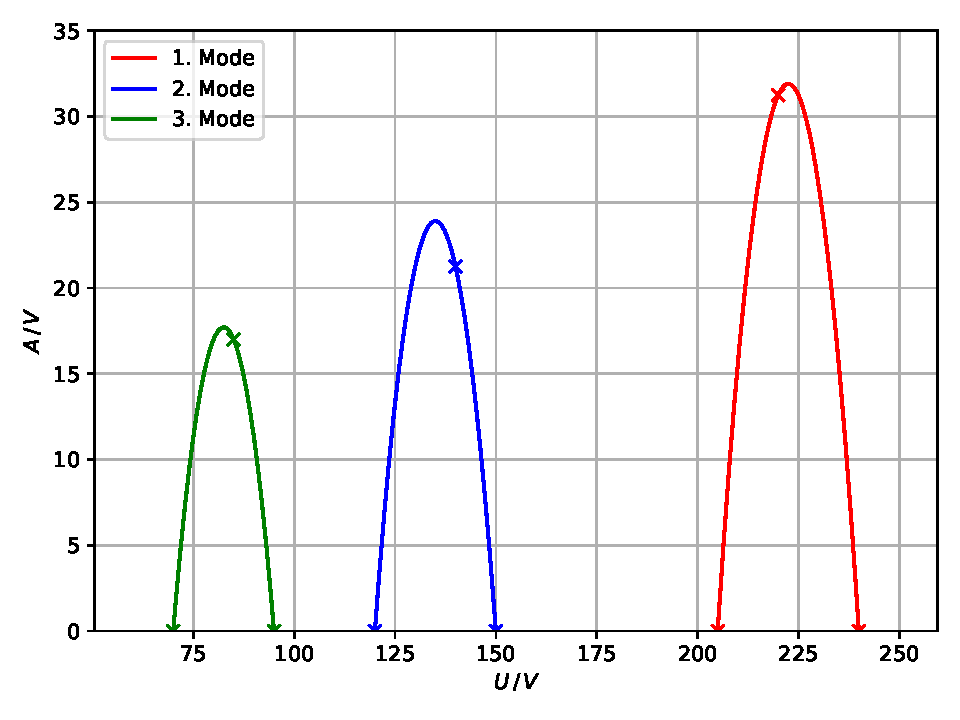
\includegraphics[width=0.8\textwidth]{content/data/moden.pdf}
    \caption{Die Messwerte $x$ mit zugehöriger Fit-Kurve (Ausgleichsparabel) für die drei Moden. \cite{matplotlib}\cite{numpy}}
    \label{fig:moden}
\end{figure}

%tabelle ergebnisse
\begin{table}
    \centering
    \caption{Die Parameter $x, y, z$, die die Ausgleichsparabel für eine Mode beschreiben.}
    \begin{tabular}{c c c c}
        \toprule
        Modennr. & $x$ & $y$ & $z$ \\
        \midrule
        1 & $-0.104$ & $46.354$ & $-5125.000$ \\
        2 & $-0.106$ & $28.688$ & $-1912.500$ \\
        3 & $-0.113$ & $18.700$ & $-753.667$ \\
        \bottomrule
    \end{tabular}
    \label{tab:moden_ergebnisse}
\end{table}

\subsection{Berechnung der Bandbreite}
Die Daten zu elektronischen Abstimmung für den höchsten Modus bei $~\SI{9000}{\mega\hertz}$ sind in \autoref{tab:elektronische_abstimmung} aufgeführt.
\begin{table}
    \centering
    \caption{Daten zur elektronischen Abstimmung mit Reflektorspannung $U$ und Frequenz $f$, wobei $a)$ den Peak, $b)$ bzw. $c)$ die hälfte des Peaks rechts bzw. links vom Maximum beschreibt.}
    \begin{tabular}{c c c c}
        \toprule
        & a) & b) & c) \\
        \midrule
        $U \,/\, \si{\volt}$ & $220$ & $210$ & $230$ \\
        $f \,/\, \si{\mega\hertz}$ & $9010$ & $8989$ & $9029$ \\
    \end{tabular}
    \label{tab:elektronische_abstimmung}
\end{table}

Die elektronische Bandbreite (siehe \autoref{sec:moden_durchfuehrung}) beträgt
\begin{equation*}
    f' - f'' = \SI{40.0}{\mega\hertz}
\end{equation*}
und die Abstimm-Empfindlichkeit liegt bei
\begin{equation*}
    \frac{f' - f''}{U' - U''} = \SI{2.0}{\frac{\mega\hertz}{\volt}} \, .
\end{equation*}

\subsection{Bestimmung der Frequenz im Hohlleiter}
Im folgenden Teil wird die Frequenz aus der Wellenlänge bestimmt.
Die Wellenlänge $\lambda_g$ ergibt sich aus dem doppelten Abstand zweier Minima bzw. Maxima und beträgt hier
\begin{align*}
    \lambda_g &= (73 - 48) \cdot 2 \si{\milli \metre} \\
    &= \SI{50}{\milli \metre} \, .
\end{align*}
Die Breite des Hohlleiters wird mit $a = \SI{22.86}{\milli \metre}$ angegeben.
Daraus folgt nach \autoref{eq:grenzwellenlaenge} und \autoref{eq:wellenlaenge_hohleiter} die Frequenz im Hohlleiter
\begin{equation*}
    f = \SI{8885}{\mega\hertz}
\end{equation*}
,wobei mit $c = 299792458$ gerechnet wird.

\subsection{Dämpfungsmessung}
In diesem Teil soll die Dämpfung in Abhängigkeit der Einstellung der Mikrometerschraube untersucht werden.
Die vom SWR-Meter aufgenommene Dämpfung $P$ und Mikrometersteinstellung ist in \autoref{tab:daempfung} aufgelistet und in \autoref{fig:daempfung} graphisch dargestellt.
Die Theorie-Kurve wird aus $10$ Punkten der Eichkurve (siehe \autoref{tab:daempfung}) mithilfe einer Ausgleichsparabel der Form
\begin{equation*}
    P_\text{eich} = a \cdot x^2 + b \cdot x + c 
\end{equation*}
bestimmt:
\begin{align*}
    a &= \SI{1.59(6)}{} \\
    b &= \SI{0.65(15)}{} \\
    c &= \SI{0.03(8)}{}
\end{align*}

Wie in der Abbildung zu erkennen ist, sind die Messwerte stark zur Eichkurve verschoben.
Es ist ein relativ konstanter Abstand zu erkennen.
Daher wird die Differenz zwischen den Messwerten und der Eichkurve berechnet und der Mittelwert gebildet
\begin{equation}
    \bar{x}_\text{Verschiebung} = \SI{14.38}{\milli\metre}
\end{equation}
und die Messwerte um diesen Wert verschoben.
\begin{table}
    \centering
    \caption{Die gemessene Dämpfung $P$ und die theoretische Dämpfung $P_\text{eich}$ als Funktion der Mikrometerablesung $x$.}
    \label{tab:daempfung}
    \begin{tabular}{S[table-format=1] S[table-format=1.2] S[table-format=1.2]}
        \toprule
        $P \,/\, \si{\dB}$ & $x \,/\, \si{\milli\metre}$ & $P_\text{eich} \,/\, \si{\dB}$\\
        \midrule
        0 & 2.8 & 0 \\
        2 & 3.05 & 0.9 \\
        4 & 3.21 & 1.4 \\
        6 & 3.4 & 1.75 \\
        8 & 3.5 & 2.05 \\
        10 & 3.7 & 2.3 \\
        \bottomrule
    \end{tabular}
\end{table}

\begin{figure}
    \centering
    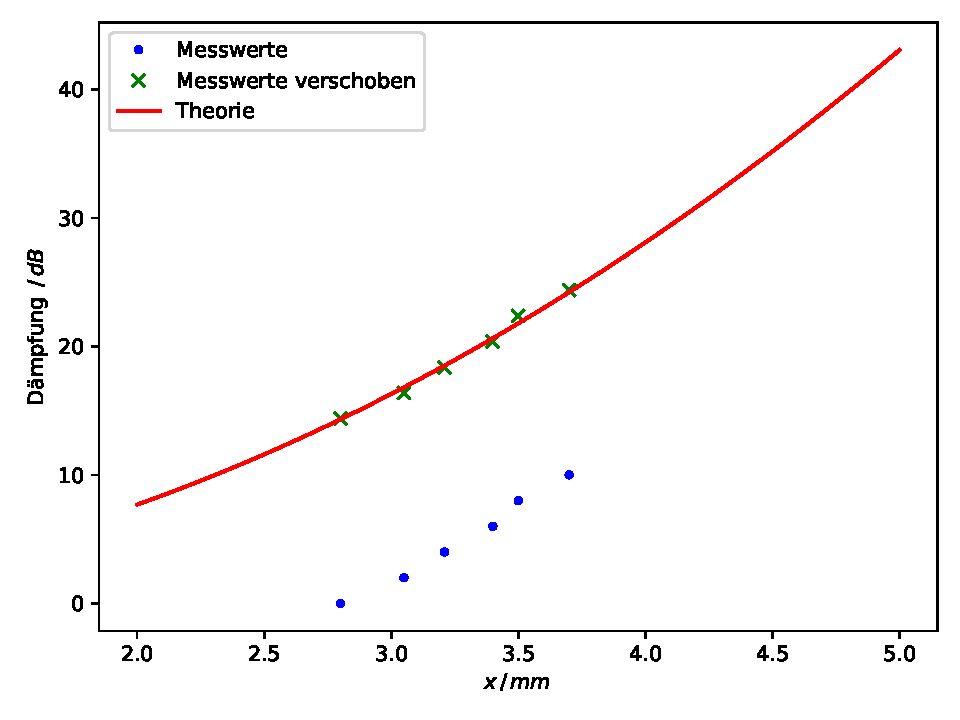
\includegraphics[width=0.8\textwidth]{content/data/daempfung.pdf}
    \caption{Die theoretische Dämpfungskurve (rot), Messwerte (blaue) und die angepassten Messwerte (grün) in Abhängigkeit der Mikrometereinstellung.}
    \label{fig:daempfung}
\end{figure}
